% =====================================================================
%  Model Scanner (Jorak) — Reference-free detection of LLM abliteration
%  SIMPLIFIED VERSION (English). Condensed mathematical justification.
%
%  COMPILE : Overleaf -> pdfLaTeX engine.
%  FIGURES : the 3 PNGs live in docs/figures/ :
%                  scatter.png, heatmap-ablated.png, heatmap-censored.png
%
%  French version : docs/report_fr.tex (kept in lockstep with this file)
% =====================================================================
\documentclass[11pt,a4paper]{article}

\usepackage[T1]{fontenc}
\usepackage[utf8]{inputenc}
\usepackage[english]{babel}
\usepackage{lmodern}
\usepackage{amsmath,amssymb,amsthm,mathtools}
\usepackage{geometry}
\geometry{margin=2.4cm}
\usepackage{booktabs}
\usepackage{array}
\usepackage{graphicx}
\usepackage{float}
\usepackage{tikz}
\graphicspath{{figures/}{./}}
\usepackage{xcolor}
\usepackage[most]{tcolorbox}
\usepackage{caption}
\usepackage{hyperref}
\hypersetup{colorlinks=true,linkcolor=blue!60!black,citecolor=blue!60!black,urlcolor=blue!60!black}

\theoremstyle{definition}
\newtheorem{definition}{Definition}
\theoremstyle{plain}
\newtheorem{proposition}{Proposition}

% --- "intuition" box (plain-language) ---
\newtcolorbox{intuition}[1][Intuition]{
  enhanced, breakable,
  colback=blue!4, colframe=blue!55!black, fonttitle=\bfseries,
  title=#1, boxrule=0.6pt, left=4pt,right=4pt,top=3pt,bottom=3pt}

% --- math shortcuts ---
\newcommand{\R}{\mathbb{R}}
\newcommand{\rhat}{\hat{r}}
\newcommand{\norm}[1]{\left\lVert #1 \right\rVert}
\newcommand{\inner}[2]{\langle #1, #2 \rangle}
\newcommand{\dmodel}{d_{\text{model}}}
\newcommand{\E}{\mathbb{E}}
\DeclareMathOperator{\proj}{proj}
\DeclareMathOperator{\tr}{tr}

\title{\textbf{Model Scanner} — the \textbf{Jorak} project \\[2mm]
\large \emph{Reference-free} detection of abliteration in large language models\\
\normalsize\emph{(simplified version — condensed mathematical justification)}}
\author{Jolan Mocanu}
\date{Version 1.0 --- July 2026}

\begin{document}
\maketitle

\begin{abstract}
\noindent
\emph{Abliteration} removes the refusal behaviour of a large language model (LLM)
\textbf{without retraining}, by deleting a single direction in the model's internal
space. Detecting that a model has been abliterated is a safety and traceability
concern. \textbf{Jorak} is a \emph{reference-free} detector (it does \textbf{not}
need the original model) built on three complementary techniques: the \emph{health}
of the refusal axis measured on activations (Cohen's $d$), a \emph{spectral
signature} of the weight matrices (SVD), and observable \emph{behaviour}. This
document condenses the mathematical justification: we formalise the abliteration
mechanism, define and \emph{comment} every metric, then validate the classifier on a
matrix of real models derived from a common base (\texttt{Qwen2.5-0.5B}). The
detector correctly classifies the three provenances and yields \textbf{no false
positive} on a merely fine-tuned model. We further confirm the weight signature on
real abliterated models in the wild --- up to \textbf{8B} and across architectures
(Granite-3.2-8B, Qwen3-VL-4B) --- both flagged with maximal confidence.
\end{abstract}

\tableofcontents
\bigskip

% =====================================================================
\section{Introduction}
% =====================================================================

\subsection{Context}
So-called \emph{aligned} LLMs are trained to \textbf{refuse} certain requests
(harmful, illegal, etc.). Arditi et~al.~\cite{arditi2024} showed that this refusal is
largely carried by a \textbf{single direction} $\rhat$ in the model's internal
representation: the projection of the internal state onto $\rhat$ is high for harmful
requests and low for harmless ones. One can then \emph{remove} refusal by deleting
that direction from the weights: this is \textbf{abliteration}~\cite{labonne2024},
now automated and applied to hundreds of ``uncensored'' models shared online.

In one sentence: the model is not retrained — the wire through which it expressed
refusal is surgically \emph{unplugged}. The model still ``knows'' a request is
harmful (its internal representation is intact) but it can no longer \emph{act} on
that knowledge.

\subsection{Problem}
Given an open-source model (often quantised, sometimes without a pedigree),
\textbf{has it been abliterated?} The core difficulty: in practice we do \emph{not}
have the original model to compare ``before/after''. We therefore want a
\emph{reference-free} detector. Comparing against the original (the ``oracle'') only
serves to \emph{validate} the method during development, never in production.

\subsection{Jorak: the project and its three techniques}
\begin{intuition}[Jorak = the project, not one metric]
\textbf{Jorak} is the name of the \emph{project} (this scanner and the report it
produces). It is not a single metric, but a \textbf{set of three} complementary
detection techniques that examine the model from three angles:
\begin{itemize}\itemsep1pt
  \item \textbf{Cohen's $d$} — on the \emph{activations}: is the refusal axis still
  \emph{alive}? (\S\ref{sec:cohen})
  \item the \textbf{SVD spectral signature} — on the \emph{weights}: is the refusal
  write-path \emph{severed}? It carries three signals, $\mathcal{A}$, $\mathcal{B}$
  and $\mathcal{S}$ (\S\ref{sec:svd}).
  \item \textbf{behaviour} — does the model still \emph{refuse}? (\S\ref{sec:behav})
\end{itemize}
In particular, the \texttt{svd\_alignment} field ($\mathcal{A}$) is \emph{only one}
of the signals of the second technique: it must not be confused with ``Jorak'' as a
whole.
\end{intuition}

\noindent These three techniques are combined by a \textbf{provenance classifier}
(\S\ref{sec:classif}) that places the model into one of four classes:
\emph{censored} / \emph{ablated} / \emph{finetuned-decensored} / \emph{ambiguous},
with a confidence score and the affected layers.

% =====================================================================
\section{Mathematical preliminaries}\label{sec:prelim}
% =====================================================================
We write $\dmodel$ for the internal dimension ($\dmodel=896$ for
\texttt{Qwen2.5-0.5B}) and $L$ for the number of layers ($L=24$ here). Vectors are
columns; $\norm{\cdot}$ is the Euclidean norm, $A^\top$ the transpose, $I$ the
identity.

\subsection{The residual stream: where representations live}
At each position a transformer maintains a vector $h\in\R^{\dmodel}$, the
\textbf{residual stream}~\cite{elhage2021}. Its key property is that it is
\textbf{additive}: every sub-module \emph{reads} $h$, computes a contribution $c$,
and \emph{adds} it ($h\leftarrow h+c$). Only two modules \emph{write} into this
stream — the attention output \texttt{o\_proj} and the MLP output
\texttt{down\_proj} — so they are the only targets of abliteration.

\begin{intuition}[Why ``directions''?]
Think of $h$ as a whiteboard onto which each layer \emph{adds} an annotation without
erasing anything. Because information is encoded largely \emph{linearly}, a concept
becomes a \textbf{direction} that can be isolated by projection — the founding
observation of mechanistic interpretability~\cite{elhage2021}.
\end{intuition}

\subsection{Projection and cosine}
For $u,v\in\R^{\dmodel}$, the inner product $\inner{u}{v}=u^\top v$ measures their
alignment. The \textbf{projection} of $v$ onto a unit direction $\rhat$
($\norm{\rhat}=1$) is $\proj_{\rhat}(v)=(\rhat\rhat^\top)v$; the matrix
$P=\rhat\rhat^\top$ is the \textbf{projector} onto the line of $\rhat$. Its
complement $I-P$ \emph{erases} the component along $\rhat$ and keeps the rest — which
is, word for word, the abliteration operation (\S\ref{sec:meca}). The angle between
two vectors is the \textbf{cosine}
$\cos(u,v)=\inner{u}{v}/(\norm{u}\,\norm{v})\in[-1,1]$; since the sign of a direction
is arbitrary, we usually work with $\lvert\cos\rvert$.

\subsection{The linear representation hypothesis}
We posit that the concept ``the request is harmful'' is encoded \textbf{linearly}:
there exists a direction $\rhat$ such that $\inner{\rhat}{h}$ is high for
\emph{harmful} examples and low for \emph{harmless} ones. This idea — from linear
regularities in word embeddings~\cite{mikolov2013} to their formalisation for
LLMs~\cite{park2023} — turns a fuzzy question (``is the model censored?'') into a
precise \emph{geometric} one, which the following linear tools answer one by one.

% =====================================================================
\section{The abliteration mechanism}\label{sec:meca}
% =====================================================================
\begin{definition}[Refusal direction]
The \textbf{refusal direction} $\rhat\in\R^{\dmodel}$, $\norm{\rhat}=1$, is the
direction of the residual stream along which the model encodes and expresses refusal.
\end{definition}

Let $W$ be a matrix that \emph{writes} into the residual stream
($W\in\{\texttt{o\_proj},\texttt{down\_proj}\}$). To prevent the model from writing
along $\rhat$, one applies $I-\rhat\rhat^\top$ to every output, i.e.\ replaces $W$ by
\begin{equation}\label{eq:ablate}
  W' = (I-\rhat\rhat^\top)\,W .
\end{equation}
This is a \textbf{rank-$1$} perturbation: the model can write anything \emph{except}
along the refusal axis.

\begin{proposition}[The invariant exploited by detection]\label{prop:invariant}
After abliteration, $\rhat^\top W'=0$: the refusal direction lies in the
\textbf{left null space} of $W'$.
\end{proposition}
\begin{proof}
$\rhat^\top W'=\rhat^\top(I-\rhat\rhat^\top)W=\rhat^\top W-(\rhat^\top\rhat)\rhat^\top W=0$,
since $\rhat^\top\rhat=1$.
\end{proof}

\noindent This invariant is \emph{exact} and \emph{permanent} (engraved in the
shipped weights). Abliteration touches only the write weights: the internal
representation of refusal is left intact. Hence the \textbf{signature} we look for:
\[
  \boxed{\ \text{refusal axis \emph{alive}}\ \wedge\ \text{write-path \emph{severed}}\ }
\]
a combination no fine-tuning reproduces: fine-tuning shifts all weights and
representations, it does not \emph{unplug} a single direction. Detecting therefore
means \emph{recovering} $\rhat$ — which we are not given — then \emph{checking} that
it is both alive in the activations and absent from the weights.

% =====================================================================
\section{Jorak's three detection techniques}\label{sec:outils}
% =====================================================================
The scanner runs a \textbf{single} forward pass (``scan-once'') and derives all
measurements from it. We work layer by layer: $h^{h}_{\ell,i}$ (resp.\
$h^{hl}_{\ell,i}$) is the internal state at the last prompt token of the
\emph{harmful} (resp.\ \emph{harmless}) example $i$ at the output of layer $\ell$,
with $n$ examples per class.

\subsection{Prerequisite: the refusal direction by mean-difference}
We do not know $\rhat$; we \emph{estimate} it. The simplest separator of two point
clouds is the vector joining their centroids:
\begin{equation}\label{eq:meandiff}
  \rhat_\ell=\frac{\mu^{h}_\ell-\mu^{hl}_\ell}{\norm{\mu^{h}_\ell-\mu^{hl}_\ell}},
  \qquad
  \mu^{h}_\ell=\tfrac1n\textstyle\sum_i h^{h}_{\ell,i},\quad
  \mu^{hl}_\ell=\tfrac1n\textstyle\sum_i h^{hl}_{\ell,i}.
\end{equation}
This is the \emph{mean-diff} direction~\cite{arditi2024}: a rank-$1$ separator, no
matrix inversion, robust on small data. It yields a per-layer \emph{candidate}
refusal axis, estimated without the original model. \emph{(Implemented in
\texttt{modelscanner/directions/mean\_diff.py}.)}

\subsection{Technique 1 — Axis health: Cohen's $d$ (activations)}\label{sec:cohen}
We project each state onto $\rhat_\ell$ ($p_{\ell,i}=\inner{\rhat_\ell}{h_{\ell,i}}$)
and quantify the \emph{separation} of the two scalar clouds (harmful vs harmless)
with Cohen's \textbf{effect size}~\cite{cohen1988}:
\begin{equation}\label{eq:cohen}
  d_\ell=\frac{\overline{p^{h}_\ell}-\overline{p^{hl}_\ell}}{\sigma_{\text{pool},\ell}},
  \qquad
  \sigma_{\text{pool}}=\sqrt{\tfrac{(n_h-1)s_h^2+(n_{hl}-1)s_{hl}^2}{n_h+n_{hl}-2}} .
\end{equation}

\begin{intuition}[What $d_\ell$ measures]
$d_\ell$ expresses ``by how many standard deviations'' the two classes are separated
along $\rhat_\ell$. Dividing by $\sigma_{\text{pool}}$ makes it \emph{dimensionless},
hence comparable across layers, models and quantisations. Usual
conventions~\cite{cohen1988}: $0.2$ small, $0.5$ medium, $0.8$ large. A large
$d_\ell$ signals an \textbf{alive axis}; we measure up to $d_\ell\approx 4.5$ in the
deep layers of \texttt{Qwen2.5-0.5B}.
\end{intuition}

\noindent\textbf{Safeguard.} Computing $\rhat$ \emph{and} $d$ on the \emph{same}
probes makes $d$ optimistic. The protocol therefore enforces a \textbf{train/test
split} of the probes (estimate $\rhat$ on one subset, measure $d$ on a disjoint one).
\emph{(Implemented in \texttt{modelscanner/metrics/axis\_health.py}.)} Cohen's $d$
measures the \emph{vitality} of the axis in the representations; it says nothing about
the weights — an abliterated model keeps a live axis while having a severed
write-path. Hence the next technique.

\subsection{Technique 2 — Spectral weight signature (SVD)}\label{sec:svd}

\paragraph{(a) Reading the direction straight from the matrix.}
A first idea would be to project \emph{our} estimated $\rhat$ onto the weights and
measure what still ``gets through''. This \textbf{fails}: our $\rhat_m$ (mean-diff) is
not exactly the direction $\rhat_a$ used by the ablator, so $\rhat_m^\top W'\neq 0$
and the residual \emph{drowns} in noise (of order $1/\sqrt{\dmodel}\approx 0.03$). We
therefore stop \emph{guessing} $\rhat$ and \emph{read} it from the matrix, via the
\textbf{singular value decomposition}~\cite{golub2013}.

\begin{intuition}[SVD in one picture]
$W$ maps the unit sphere to an \emph{ellipsoid}. Its axis lengths are the
\textbf{singular values} $\sigma_1\ge\dots\ge\sigma_r\ge 0$, and their output
directions are the \textbf{left singular vectors} $u_1,\dots,u_r$. The smallest one,
$u_{\min}$, is the direction the matrix ``produces least''.
\end{intuition}

\noindent Formally $W=U\Sigma V^\top$, and $\norm{u_i^\top W}=\sigma_i$.
\textbf{Consequence (the heart of the method)}: after abliteration $\rhat_a^\top W'=0$
(Prop.~\ref{prop:invariant}), so $\rhat_a$ is a left singular vector with
\emph{zero} singular value: $u_{\min}(W')\approx\rhat_a$. \emph{We recover the
ablated direction without ever having known it.}

\paragraph{(b) Signal $\mathcal{A}$ — cross-layer alignment (the smoking gun).}
A single layer is not enough (every matrix has a $u_{\min}$). The decisive signature
is that, on an abliterated model, \emph{all} layers share the \emph{same}
$u_{\min}\approx\rhat_a$ (the same direction having been removed everywhere). We stack
the $u_{\min}$ into $\mathbf{U}\in\R^{L\times\dmodel}$ (unit rows) and measure their
coherence:
\begin{equation}\label{eq:align}
  \mathcal{A}=\frac{\sigma_1(\mathbf{U})}{\norm{\mathbf{U}}_F}\in\Big[\tfrac{1}{\sqrt{L}},\,1\Big].
\end{equation}

\begin{intuition}[Reading $\mathcal{A}$]
If all layers share the same direction, $\mathbf{U}$ is rank $1$ and
$\mathcal{A}\approx 1$. If the directions are unrelated (uncorrelated noise of a
healthy model), $\mathcal{A}\approx 1/\sqrt{L}$. With $L=24$ this gives $\approx 0.20$
(healthy) versus $\approx 0.90$ (ablated): a sharp separation, \emph{independent of
any probe}, computable on CPU. We also keep a \textbf{per-layer signal}
$a_\ell=\lvert\cos(u_{\min}^{(\ell)},w)\rvert$ ($w$~=~dominant shared axis) to tell
\emph{which} layers were touched (heatmap rows).
\end{intuition}

\paragraph{(c) Signal $\mathcal{B}$ — \emph{band} alignment (localized ablation).}
$\mathcal{A}$ averages over \emph{all} layers. But a \emph{stealthy} ablation
(Heretic-style, optimised to preserve capabilities) touches only a band of layers:
the global average is then \emph{diluted} and slips back below threshold. We add a
\emph{per-band} statistic:
\begin{equation}\label{eq:band}
  \mathcal{B}=\max_{0\le i\le L-w}\ \frac1w\sum_{\ell=i}^{i+w-1} a_\ell ,
  \qquad w\approx L/6 ,
\end{equation}
the maximal mean of the per-layer alignment over a window of $w$ \emph{consecutive}
layers. $\mathcal{B}$ is \emph{position-agnostic}: a healthy model (scattered noise)
forms no band ($\mathcal{B}$ low); a localized ablation (a contiguous band) gives a
high $\mathcal{B}$, wherever it sits.

\paragraph{(d) Signal $\mathcal{S}$ — \emph{subspace} alignment (multi-direction).}
$\mathcal{A}$ and $\mathcal{B}$ assume a \emph{single} removed direction. But,
empirically, refusal lives in \emph{several} independent directions, even a
\emph{concept cone}~\cite{wollschlager2025,piras2025}, and recent ablators
(Gabliteration~\cite{gabliteration}) remove a \emph{subspace} of $k>1$
directions: the trace is then \emph{spread} over the $k$ smallest singular values and
no single $u_{\min}$ is shared. We therefore \emph{generalise} to the low-rank
subspace. Let $B_\ell\in\R^{\dmodel\times k}$ be the $k$ left singular vectors of
smallest singular value at layer $\ell$; we seek the most \emph{shared} $k$-D
subspace:
\begin{equation}\label{eq:subspace}
  M=\sum_{\ell=1}^{L} B_\ell B_\ell^\top,\qquad
  \mathcal{S}=\frac{1}{Lk}\sum_{i=1}^{k}\lambda_i(M)\ \in\Big[\tfrac{k}{\dmodel},\,1\Big],
\end{equation}
where $\lambda_1\ge\dots$ are the eigenvalues of $M$. $\mathcal{S}\to 1$ if all layers
share the same $k$-D subspace (multi-direction ablation);
$\mathcal{S}\approx k/\dmodel$ if the subspaces are unrelated (healthy). For $k=1$,
$\mathcal{S}=\mathcal{A}^2$: it is indeed a generalisation.

\begin{intuition}[The three weight signals at a glance]
$\mathcal{A}$ detects \emph{total} ablation (all layers); $\mathcal{B}$ the
\emph{localized} ablation (a band of layers); $\mathcal{S}$ the
\emph{multi-direction} ablation (a subspace of $k$ directions). The
``weights severed'' criterion is: \textbf{$\mathcal{A}$, $\mathcal{B}$ \emph{or}
$\mathcal{S}\ge 0.5$}. \emph{(All computed in pure NumPy, without inference, in
\texttt{modelscanner/metrics/jorak.py} — the \emph{reference-free}, CPU core of Jorak.)}
\end{intuition}

\subsection{Technique 3 — Behaviour}\label{sec:behav}
We make the model \emph{generate} a reply to harmful prompts and measure the
\textbf{refusal rate} by marker matching (``I cannot'', ``sorry'', \dots) — the
standard evaluation heuristic~\cite{zou2023}. This is the \emph{only} signal that
tells a model that \emph{refuses} from one that \emph{complies}.

\begin{intuition}[Why behaviour is indispensable]
A merely \emph{finetuned-decensored} model also keeps an \emph{alive} axis (high $d$)
\emph{and} \emph{intact} weights ($\mathcal{A},\mathcal{B},\mathcal{S}$ low): on
activations and weights alone it is \textbf{indistinguishable} from a censored model.
Only \emph{behaviour} separates them — the censored one refuses, the finetuned one
complies. The behavioural plan is therefore not optional.
\end{intuition}

\noindent We additionally measure \textbf{harmless over-refusal} (refusing
\emph{innocuous} requests) and \textbf{multilingual asymmetry} (refusal gap across
languages): two \emph{damage} markers. A cleanly finetuned model stays consistent; an
ablation, by contrast, damages behaviour (over-refusal, uneven refusal across
languages). \emph{(Implemented in \texttt{modelscanner/metrics/behavioral.py}.)}

\subsection{The provenance classifier}\label{sec:classif}
We combine the scalar indicators (calibrated thresholds): \emph{alive axis}
($\max_\ell d_\ell\ge 1$), \emph{weights severed} ($\mathcal{A}$, $\mathcal{B}$
\textbf{or} $\mathcal{S}\ge 0.5$), \emph{complies} (refusal rate $<0.5$). The rule:
\[
\begin{array}{l@{\quad}l}
  \text{weights severed} & \Rightarrow \textbf{ABLATED}\ (\text{alive axis expected})\\
  \text{else, refuses} & \Rightarrow \textbf{CENSORED}\\
  \text{else, complies} & \Rightarrow \textbf{FINETUNED-DECENSORED}\\
  \text{inconsistent} & \Rightarrow \textbf{AMBIGUOUS}
\end{array}
\]
We can visualise the rule on a \textbf{provenance plane}: $\mathcal{A}$ on the
$x$-axis (weights severed $\rightarrow$), refusal rate on the $y$-axis ($\uparrow$
refuses). Weight severance ($x$) isolates the ablated model; behaviour ($y$)
separates censored from finetuned. The \textbf{confidence} returned is the
\emph{margin} of the deciding signal (its distance to threshold).

\paragraph{On the thresholds.} The decision thresholds are \emph{principled
defaults}, not values fitted to the test bench. For the weight signals, $0.5$ is the
midpoint between the theoretical floor of an uncorrelated model
($1/\sqrt{L}\approx 0.2$ for $L=24$) and the rank-$1$ ceiling ($1$); for axis health,
$d\ge 1$ follows Cohen's ``large effect'' convention~\cite{cohen1988}; for behaviour,
refusal~$<0.5$ is the natural majority split. A systematic per-signal sweep (ROC) is
left as future work --- the margins reported in \S\ref{sec:resultats} show the current
defaults sit far from the decision boundary.

\paragraph{Anti-false-positive guard (behavioural veto).} The rule above has one
crucial exception, learned from the $8$B campaign: if the weights look severed
\emph{but} the model \textbf{still refuses broadly} (refusal rate $\ge 0.5$),
\emph{behaviour wins} and the verdict stays \textbf{CENSORED}. A weight signal can be
a \emph{false positive} (e.g.\ a naturally aligned band on a base model); a
successful ablation, by contrast, \emph{complies} by construction and never triggers
this veto.

\begin{intuition}[The stealthy case, in brief]
A \emph{multi-direction norm-preserving} ablation can leave the weights ``intact'' to
the SVD ($\mathcal{A},\mathcal{B},\mathcal{S}$ below threshold). Behaviour then betrays
it: a \emph{strongly} alive axis combined with compliance and incoherent damage
(over-refusal / multilingual asymmetry) cannot be explained by a clean fine-tune. The
returned confidence is more \emph{moderate}, because the evidence is \emph{indirect}.
\end{intuition}

\noindent\emph{(Implemented in \texttt{modelscanner/classifier/scanner.py}:
\texttt{classify(...)} is a pure function, testable without a model; \texttt{scan(model)}
orchestrates the scan-once and assembles a \texttt{ScanResult}.)}

% =====================================================================
\section{Results}\label{sec:resultats}
% =====================================================================
\textbf{Test bench.} Three models derived from the \emph{same} \texttt{Qwen2.5-0.5B}
base (same architecture, same size — a clean comparison):
\texttt{Qwen2.5-0.5B-Instruct} (\emph{censored}),
\texttt{huihui-ai/\dots-abliterated} (real \emph{ablated}),
\texttt{dphn/Dolphin3.0-Qwen2.5-0.5B} (\emph{finetuned-decensored}, the false
positive to avoid), plus a real Heretic (a \emph{localized} ablation).
\textbf{Probes}: $40$ harmful/harmless pairs matched in length and register; with a
train/test split.

\begin{table}[H]
\centering
\caption{Scanner verdict on the matrix. $\mathcal{A}$: global SVD alignment;
$\mathcal{B}$: band alignment (localized); $\mathcal{S}$: subspace alignment
($k{=}4$); $d_{\max}$: axis health; ``refusal'': refusal rate.}
\label{tab:matrice}
\begin{tabular}{llccccc}
\toprule
Model & Label & $d_{\max}$ & $\mathcal{A}$ & $\mathcal{B}$ & $\mathcal{S}$ & refusal \\
\midrule
\texttt{Qwen2.5-0.5B-Instruct} & \textsc{censored} & $4.5$ & $0.24$ & $0.28$ & $0.08$ & $0.88$ \\
\texttt{huihui\dots abliterated} & \textsc{ablated} & $2.6$ & $\mathbf{0.90}$ & $\mathbf{0.99}$ & $0.29$ & $0.06$ \\
\texttt{grisun0\dots heretic} & \textsc{ablated} & $3.3$ & $0.29$ & $\mathbf{0.67}$ & $0.10$ & --- \\
\texttt{Dolphin3.0-Qwen2.5-0.5B} & \textsc{finetuned} & $3.0$ & $0.24$ & $0.28$ & $0.08$ & $0.06$ \\
\bottomrule
\end{tabular}
\end{table}

\noindent\emph{\small Reproduce: \texttt{modelscanner scan <model> --behavioral
--report}; every value is read verbatim from the emitted \texttt{scan\_log.json}
(probe set: $40$ harmful/harmless pairs, train/test split).}

\noindent All four provenances are \textbf{correctly classified}, and the finetuned
model is \textbf{not} mistaken for an ablated one (the critical false positive is
avoided). Three readings summarise the matrix:
\begin{itemize}\itemsep2pt
  \item \textbf{SVD is the real smoking gun.} Only $\mathcal{A}$ separates the ablated
  model ($0.90$) from the rest ($0.24$). The naive projection of $\rhat$ onto the
  weights is $\approx 0.038$ \emph{for all three} models (= the random floor $0.033$):
  it sees nothing. It is the \emph{spectral} signature that decides.
  \item \textbf{Behaviour separates what the weights cannot.} The finetuned model has
  an alive axis ($d_{\max}=3.0$) and intact weights ($\mathcal{A}=0.24$): identical to
  the censored one under reference-free signals. Only the refusal rate tells them
  apart ($0.06$ vs $0.88$).
  \item \textbf{The band catches the localized ablation.} The Heretic model has
  $\mathcal{A}=0.29$ (below threshold: the global signal would \emph{miss} it), but
  $\mathcal{B}=0.67$: Heretic touched only a \emph{deep} band (layers $19$--$22$ of
  $24$), revealed by the sliding window.
\end{itemize}
The $\mathcal{S}$ column stays \emph{dormant} ($\le 0.29$) on these
\emph{single}-direction ablations: by construction it only fires on
\emph{multi}-direction ablation, and introduces no false positive here.

\begin{figure}[H]
\centering
\includegraphics[width=0.72\linewidth]{scatter.png}
\caption{\textbf{Provenance plane.} $x$-axis: SVD alignment $\mathcal{A}$ (weights
severed $\rightarrow$). $y$-axis: refusal rate ($\uparrow$ refuses). The three models
occupy three distinct quadrants, matching exactly their provenance.}
\label{fig:scatter}
\end{figure}

\begin{figure}[H]
\centering
\includegraphics[width=0.9\linewidth]{heatmap-ablated.png}
\caption{\textbf{Per-layer signature of the ablated model.} The \emph{per-layer weight
alignment} row $a_\ell$ (scale $[0,1]$) is \textbf{saturated} on almost every layer:
the ablation touched the whole network.}
\label{fig:heatmap-abl}
\end{figure}

\begin{figure}[H]
\centering
\includegraphics[width=0.9\linewidth]{heatmap-censored.png}
\caption{\textbf{Censored model (control).} On the same $[0,1]$ scale, the
\emph{per-layer weight alignment} row stays \textbf{dark} ($\approx 0.2$): no shared
direction was removed.}
\label{fig:heatmap-cen}
\end{figure}

\noindent\textbf{Confidence.} The verdict confidence is the \emph{margin} of the
deciding signal: $0.81$ (ablated), $0.75$ (censored), $0.88$ (finetuned).

\subsection{Field validation at scale and across architectures}
Beyond the controlled $0.5$B bench, we ran Jorak on real abliterated models released
online, at larger scale and on different architectures (Table~\ref{tab:field}). Both
are correctly flagged \textsc{abliterated} at \textbf{maximal confidence}; for Granite
the verdict matches the declared provenance (\emph{expected}~$\checkmark$).

\begin{table}[H]\centering
\caption{Field validation on real abliterated models (huihui lineage). Values read
from each model's \texttt{scan\_log.json}.}
\label{tab:field}
\begin{tabular}{llccccc}
\toprule
Model & Arch\,·\,size & $\mathcal{A}$ & $\mathcal{B}$ & $\mathcal{S}_{k=4}$ & $d_{\max}$ & refusal \\
\midrule
\texttt{Qwen3-VL-4B-abliterated} & qwen3\_vl · 4B & $1.00$ & $1.00$ & $0.39$ & $4.97$ & $0.00$ \\
\texttt{granite-3.2-8B-abliterated} & granite · 8B & $0.99$ & $1.00$ & $0.50$ & $5.07$ & $0.06$ \\
\bottomrule
\end{tabular}
\end{table}

\noindent Three takeaways: \textbf{(i)} the cross-layer signature $\mathcal{A}$
\emph{saturates} ($0.99$--$1.00$) at $8$B and on a vision--language model --- it is
not an artefact of the $0.5$B setting; \textbf{(ii)} the smoking-gun combination --- a
\emph{live} axis ($d_{\max}\approx 5$) with a \emph{severed} write-path and
\emph{compliance} (refusal~$\approx 0$) --- holds at scale; \textbf{(iii)} capability
stays largely intact (Granite: factual accuracy $0.88$, perplexity $11.2$), i.e.\ a
\emph{clean} ablation that the weight plane nonetheless detects outright.

\begin{figure}[H]\centering
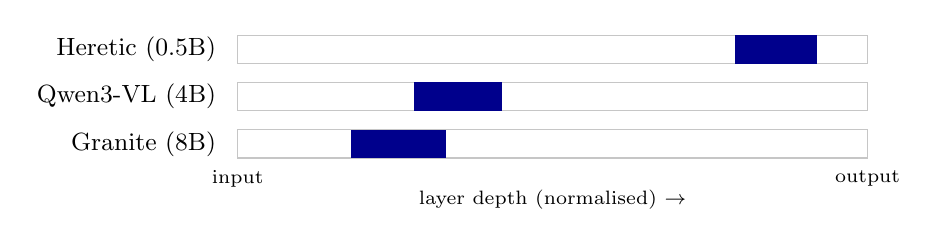
\begin{tikzpicture}[yscale=0.6]
\foreach \name/\y/\a/\b in {%
  Heretic (0.5B)/2/0.79/0.92,
  Qwen3-VL (4B)/1/0.28/0.42,
  Granite (8B)/0/0.18/0.33}{
  \draw[gray!45] (0,\y) rectangle (8,\y+0.6);
  \fill[blue!55!black] (8*\a,\y) rectangle (8*\b,\y+0.6);
  \node[left] at (-0.15,\y+0.3) {\small \name};
}
\node[below] at (0,-0.05) {\scriptsize input};
\node[below] at (8,-0.05) {\scriptsize output};
\node[below=7pt] at (4,-0.05) {\scriptsize layer depth (normalised) $\rightarrow$};
\end{tikzpicture}
\caption{\textbf{The band signal $\mathcal{B}$ is position-agnostic.} The contiguous
band of severed layers (shaded) sits at a \emph{different} depth for each model ---
deep for Heretic, mid for Qwen3-VL and Granite --- yet the sliding window
(Eq.~\eqref{eq:band}) catches it in every case.}
\label{fig:band}
\end{figure}

\paragraph{Honest scope.} These two models are \emph{positives} (both ablated). A full
$8$B matrix with \emph{negative controls} (a censored and a finetuned-only $8$B) is
left as future work; the \emph{no-false-positive} property is therefore established on
the $0.5$B matrix (\S\ref{sec:resultats}) and not yet at $8$B. The sample also covers a
single lineage/tool (huihui).

\paragraph{Methodological lesson (anti-false-positive).} The \texttt{down\_proj} (MLP
output) target has a band $\mathcal{B}$ that is \emph{naturally high on base models}
(non-discriminative) and produced false positives in an early multi-target attempt;
the campaign verdict therefore relies on \texttt{o\_proj} alone, backed by the
behavioural veto (\S\ref{sec:classif}). The scan log now records the \emph{per-target
breakdown} ($\mathcal{A}$, $\mathcal{B}$ for \texttt{o\_proj}/\texttt{down\_proj}
separately) so any re-examination is unambiguous.

% =====================================================================
\section{Related work}\label{sec:related}
% =====================================================================
Jorak sits at the crossing of three recent strands: the \emph{geometry} of refusal,
\emph{defences} against abliteration, and the \emph{landscape} of ablation tools.

\paragraph{From a single mechanism to multiple directions.}
The starting point — a \emph{single} refusal direction~\cite{arditi2024} — has been
qualified. Wollschläger et~al.~\cite{wollschlager2025} show, via a gradient-based
approach, the existence of \emph{several} mechanistically independent directions, even
multi-dimensional \emph{concept cones}, and that orthogonality does not imply
independence under intervention. Piras et~al.~\cite{piras2025} likewise extract
multiple directions via Self-Organizing Maps (SOM) and establish that ablating
\emph{several} directions suppresses refusal more effectively than one (their method in
fact \emph{generalises} the mean-difference of Eq.~\eqref{eq:meandiff}). Zhang \&
Sun~\cite{zhang2025dbdi} finally split the single direction into two processes —
\emph{harm detection} and \emph{refusal execution}. These results directly motivate our
\emph{subspace} signal $\mathcal{S}$ (\S\ref{sec:svd}d): one cannot assume a single
$u_{\min}$ carries the whole ablation trace.

\paragraph{Attack, defence, detection.}
Abliteration has prompted its own \emph{defences}. Abu Shairah et~al.~\cite{abushairah2025}
propose an \emph{extended-refusal} fine-tune (the model \emph{justifies} its refusal)
that keeps the post-attack refusal drop to at most $10\%$, versus $70$--$80\%$ for the
baseline. Jorak is \emph{complementary}: not a defence but a \emph{detection}/forensic
tool. Notably, such a defended model \emph{still refuses} after an ablation attempt —
precisely the case our \emph{behavioural veto} (\S\ref{sec:classif}) is designed not to
mistake for a healthy model.

\paragraph{The abliteration tool landscape.}
Young~\cite{young2025} benchmarks four abliteration tools (Heretic, DECCP, ErisForge,
FailSpy) across sixteen instruct models ($7$--$14$B) and confirms that capability
damage is tool-dependent, with mathematical reasoning (GSM8K) the most sensitive —
which supports both our multi-tool campaign (\S\ref{sec:resultats}) and our
\emph{damage markers} (over-refusal, asymmetry). Finally, recent
\emph{norm-preserving} methods~\cite{dang2026,grimjim}, which replace ``binary''
ablation with a norm-preserving rotation, are exactly the class of \emph{stealthy}
ablation we list as an open limitation (\S\ref{sec:robustesse}).

% =====================================================================
\section{Robustness and limitations}\label{sec:robustesse}
% =====================================================================
\begin{itemize}\itemsep2pt
  \item \textbf{Quantisation.} $\mathcal{A}$ is a \emph{cross-layer} signature; since
  quantisation noise is largely uncorrelated across layers, it barely degrades a
  \emph{shared} coherence. We conjecture the signature survives down to $4$ bits (with
  a slightly shifting, ``quant-aware'' threshold) — to be validated on \texttt{bf16},
  \texttt{bnb-4bit}, GGUF.
  \item \textbf{Ablation sophistication.} The localized ablation is covered by
  $\mathcal{B}$; the multi-direction one by $\mathcal{S}$ and, failing that, by the
  behavioural relay. Still open: \emph{partial} projection ($\alpha<1$, which makes
  $\mathcal{A},\mathcal{B},\mathcal{S}$ decrease continuously) and \emph{row-wise}
  norm-preserving~\cite{dang2026,grimjim}, which \emph{moves} the left null space and attenuates
  $\mathcal{S}$.
  \item \textbf{Architectures and formats.} MoE / MLA models need per-expert handling;
  for non-executable GGUF formats the activation plan is unavailable (fall back to
  weights $+$ behaviour).
\end{itemize}

% =====================================================================
\section{Conclusion}
% =====================================================================
The thread is simple: \emph{refusal is a direction}; \emph{abliteration erases that
direction from the write weights}, leaving an exact invariant ($\rhat^\top W'=0$);
this invariant can be \emph{read} from the matrix spectrum — without knowing the
direction or the original model — via the \textbf{alignment of the smallest singular
vectors}. Jorak combines three techniques — \emph{axis health} (Cohen's $d$), the
\emph{spectral signature} of the weights ($\mathcal{A},\mathcal{B},\mathcal{S}$) and
\emph{behaviour} — to place a model among four provenances. On a matrix of real
models, the detector classifies the three provenances correctly and avoids the
critical false positive. The whole approach is implemented and reproducible in the
\texttt{modelscanner} library.

% =====================================================================
\begin{thebibliography}{99}
\bibitem{arditi2024} A.~Arditi \emph{et al.}, \emph{Refusal in Language Models Is
Mediated by a Single Direction}, arXiv:2406.11717, 2024.
\bibitem{labonne2024} M.~Labonne, \emph{Uncensor any LLM with abliteration},
Hugging Face Blog, 2024.
\bibitem{elhage2021} N.~Elhage \emph{et al.}, \emph{A Mathematical Framework for
Transformer Circuits}, Transformer Circuits Thread (Anthropic), 2021.
\bibitem{mikolov2013} T.~Mikolov, W.~Yih, G.~Zweig, \emph{Linguistic Regularities
in Continuous Space Word Representations}, NAACL-HLT, 2013.
\bibitem{park2023} K.~Park, Y.~J.~Choe, V.~Veitch, \emph{The Linear Representation
Hypothesis and the Geometry of Large Language Models}, arXiv:2311.03658, 2023.
\bibitem{cohen1988} J.~Cohen, \emph{Statistical Power Analysis for the Behavioral
Sciences}, 2nd ed., Lawrence Erlbaum, 1988.
\bibitem{golub2013} G.~H.~Golub, C.~F.~Van~Loan, \emph{Matrix Computations},
4th ed., Johns Hopkins University Press, 2013.
\bibitem{zou2023} A.~Zou \emph{et al.}, \emph{Universal and Transferable Adversarial
Attacks on Aligned Language Models}, arXiv:2307.15043, 2023.
\bibitem{gabliteration} G.~Gülmez, \emph{Gabliteration: Adaptive Multi-Directional
Neural Weight Modification for Selective Behavioral Alteration in Large Language
Models}, arXiv:2512.18901, 2025.
\bibitem{grimjim} grimjim, \emph{Norm-Preserving Biprojected Abliteration},
Hugging Face, 2025.
\bibitem{wollschlager2025} T.~Wollschläger, J.~Elstner, S.~Geisler, V.~Cohen-Addad,
S.~Günnemann, J.~Gasteiger, \emph{The Geometry of Refusal in Large Language Models:
Concept Cones and Representational Independence}, arXiv:2502.17420, 2025.
\bibitem{piras2025} G.~Piras, R.~Mura, F.~Brau, L.~Oneto, F.~Roli, B.~Biggio,
\emph{SOM Directions are Better than One: Multi-Directional Refusal Suppression in
Language Models}, arXiv:2511.08379, 2025.
\bibitem{zhang2025dbdi} P.~Zhang, P.~Sun, \emph{Differentiated Directional
Intervention: A Framework for Evading LLM Safety Alignment}, arXiv:2511.06852, 2025.
\bibitem{abushairah2025} H.~Abu~Shairah, H.~A.~K.~Hammoud, B.~Ghanem, G.~Turkiyyah,
\emph{An Embarrassingly Simple Defense Against LLM Abliteration Attacks},
arXiv:2505.19056, 2025.
\bibitem{young2025} R.~J.~Young, \emph{Comparative Analysis of LLM Abliteration
Methods: A Cross-Architecture Evaluation}, arXiv:2512.13655, 2025.
\bibitem{dang2026} Q.-A.~Dang, C.~Ngo, \emph{Selective Steering: Norm-Preserving
Control Through Discriminative Layer Selection}, arXiv:2601.19375, 2026.
\end{thebibliography}

\end{document}
